%试卷模板
\documentclass[a3paper,twocolumn,2twoside,landscape,12pt,UTF8]{ctexart}
\usepackage{latexexercise0}
%教案模板
%\documentclass[12pt,UTF8]{ctexart}
%\usepackage{latexexercise}
\usepackage{QingDa}
\usepackage{multirow}
%\usepackage{subfig}
\usepackage[hypcap=true,labelsep=period,font=small]{caption}% 图的标题设置Fig.
\usepackage[hypcap=true]{subcaption}%用于画子图 可以适配hyperref包
\usepackage{float}

\pgfplotsset{width=6cm,compat=1.15}
\newcommand\putfig[2]{\begin{tabular}[t]{@{}l@{}}#1\\#2\end{tabular}}
\begin{document}

% \Grade{高一}
%\Name{1v2}\FirstTime{20181028}\CurrentTime{20181117}
\Name{林叶}\FirstTime{20180908}\CurrentTime{20181125}
% \Name{郭文镔}\FirstTime{20181111}\CurrentTime{20181117}
% \Name{马灿威}\FirstTime{20181111}\CurrentTime{20181111}
\Topic{任意角、弧度制与三角函数}
\Teach{任意角的三角函数}
\makefront
\vspace{-1.5em}
\startexercise
\hspace{-2.5em}
{\hei 本章节学习内容}\par
1. 建立一般三角函数的概念,并研究函数性质,包括周期性、奇偶性、单调性与最值;\par
2. 探索和研究三角函数之间的一些恒等关系;\par
3. 利用三角函数构建数学模型,解决实际问题。\par

\section{任意角与弧度制}
\subsection{预备知识}
1. 角与角度的概念;集合的表示;不等式的基本性质;集合的运算;直线的倾斜角;\par
2. 角度制;圆心角的性质;比例、分数的性质;圆的周长与面积;弦长的计算;锐角三角函数;二次函数最值/基本不等式.\par
\subsection{问题导学}
{\heiti 【思考1】}:角的概念是怎么产生的?我们生活中在什么时候用到过角的概念?\par
\vspace{6em}
{\heiti 【思考2】}:我们学过的角的定义是?能说出为什么这样定义么?这样定义的角可以应用在哪里呢?\par
\vspace{10em}
{\heiti 【思考3】}:为什么要定义角度?我们学过的角度是如何定义的?角度如何运算?\par
\vspace{10em}
\subsection{知识介绍}
生活中有许多“角”的形象,比如墙角的形状,斜坡,跷跷板,道路的转向,等等。把这些图像的共性抽象出来,就形成了角的最直观形象:\par
{\bf 角的静态定义}:具有公共端点的两条射线组成的图形叫做角。这个公共端点叫做角的顶点,这两条射线叫做角的两条边.\\
\begin{figure}[!htbp]
  \centering
  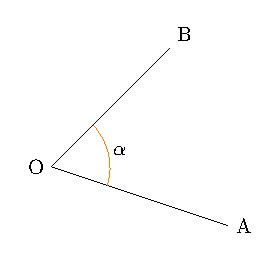
\includegraphics[scale=0.8]{Fig.ArbitraryAngle.pdf}
\end{figure}\par
{\bf 角的符号表示}:上图所示的角可记为“角AOB”、“$\angle{AOB}$”或“$\angle O$”、“角$\alpha$”或“$\angle\alpha$”
“$\alpha$”.\\
三个特殊角:{\bf\kaishu 零角,平角,直角}\par
\begin{exercise}{习题}
\item
下列说法正确的是\xz
\xx{终边相同的角一定相等}
{钝角一定是第二象限角}
{第一象限角一定不是负角}
{小于90\textdegree 的角都是锐角}
\begin{answer}B\end{answer}
\end{exercise}

\section{任意角的三角函数}
\subsection{预备知识}
1. 锐角三角函数;函数定义域
2. 勾股定理;开方;代数式化简,完全平方公式;一元二次方程求解
\subsection{问题导学}
{\heiti 【思考1】}:锐角三角函数的定义是?为什么要定义三角函数呢?三角函数有哪些应用?\par
\vspace{12em}
{\heiti 【思考2】}:锐角三角函数之间有什么关系呢?\par
\vspace{12em}

% \section{课后作业}


\stoptexercise

% sty文件使用 \RequirePackage{latexexercise0}
% 主文件使用 \documentclass[a3paper,twocolumn,2twoside,landscape,12pt,UTF8]{ctexart}
\hspace{3cm}\\
\vspace{0.5cm}
\centering{\heiti \xiaoer 福州八中2018-2019学年第一学期期中考试}\\
\vspace{0.5cm}
\centering{\heiti \erhao 高一数学\quad 必修一}\\
\vspace{0.4cm}
\centering{\wuhao 考试时间:120分钟\hspace{5em}试卷满分:150分}\\
\vspace{-1.6em}
\part{第I卷}
\vspace{-3em}
\startexercise
\begin{exercise}
\section{选择题(本大题共10小题,每小题5分,共50分.每题有且只有一个选项是正确的,请把答案填在答卷相应位置上)}
\item
设集合$A=\{x\in\mathbb{Q}|x>1\}$,则\xz
  \xx{$\varnothing\in A$}
  {$\sqrt2\notin A$}
  {$\sqrt2\in A$}
  {$\{\sqrt2\}\subseteq A$}
\begin{answer}
  B
\end{answer}
\item
下列函数中与函数$y=x(x\geq 0)$有相同图像的一个是\xz
  \xx{$\displaystyle y=\frac{x^2}x $}
  {$y=\sqrt{x^2}$}
  {$y=\sqrt[3]{x^3}$}
  {$y=(\displaystyle \sqrt x)^2 $}
\begin{answer}
  D
\end{answer}
\item
下列函数在区间$(0,+\infty) $上是增函数的是\xz
  \xx{$y=\ln(x+1)$}
  {$y=(x-1)^2$}
  {$y=x^{-2}$}
  {$y=3^{-x}$}
\begin{answer}
  A
\end{answer}
\item
设$f(x)=\begin{cases}
  x-2,x\geq10\\f[f(x+6)],x<10
\end{cases}$,则$f(9)$的值为\xz
  \xx{10}{11}{12}{13}
\begin{answer}
  B
\end{answer}
\item
若函数$f(x)=x^3+x^2-2x-2$的一个正数零点附近的函数用二分法计算,其参考数据如下:\\
\begin{center}
  \begin{tabular}{|c|c|c|}
    \hline
    $f(1)=-2$&$f(1.5)=0.625$&$f(1.25)=-0.984$\\
    \hline
    $f(1.375)=-0.260$&$f(1.4375)=0.162$&$f(1.40625)=-0.054$\\
    \hline
  \end{tabular}\\
\end{center}
那么方程$x^3+x^2-2x-2=0$的一个近似根(精确度$0.1$)是\xz
  \xx{1.2}
  {1.3}
  {1.4}
  {1.5}
\begin{answer}
  C
\end{answer}
\item
已知函数$f(x)$的值域为$[-2,3]$,则函数$f(x-2)$的值域为\xz
  \xx{$[-4,1]$}
  {$[0,5]$}
  {{$[-4,1]\cup[0,5]$}}
  {$[-2,3]$}
\begin{answer}
  A
\end{answer}
\item
三个数$0.8^9,9^{0.8},\log_{0.8}9$的大小关系为\xz
  \xx{$\log_{0.8}9<0.8^9<9^{0.8}$}
  {$0.8^9<9^{0.8}<\log_{0.8}9$}
  {$\log_{0.8}9<9^{0.8}<0.8^9$}
  {$0.8^9<\log_{0.8}9<9^{0.8}$}
\begin{answer}
  A
\end{answer}
\item
函数$f(x)=1+\log_2x$与$g(x)=2^{-(x-1)}$在同一直角坐标系下的图像大致是\xz
\begin{tikzpicture}
  \coordinate[label=below left:$O$] (O) at(0,0);
  \draw[->,>=latex](-0.8,0)--(3.6,0)node[below](x){$x$};
  \draw[->,>=latex](0,-1.5)--(0,3.2)node[left](y){$y$};
  \draw[domain=0.4:3]plot(\x,{log2(\x)});
  \draw[domain=-0.5:3]plot(\x,{pow(2,1-\x)});
  \draw[dashed](1,0.1)--(1,0)node[below](x1){$ 1 $};
  \draw[dashed](2,0.1)--(2,0)node[below](x2){$ 2 $};
  \draw[dashed](0.1,1)--(0,1)node[left](y1){$ 1 $};
  \draw[dashed](0.1,2)--(0,2)node[left](y2){$ 2 $};
  \coordinate[label=$\mathrm{A}$](a) at(1.5,-2);
  \begin{scope}[xshift=4.7 cm]
    \coordinate[label=below left:$O$] (O) at(0,0);
    \draw[->,>=latex](-0.8,0)--(3.6,0)node[below](x){$x$};
    \draw[->,>=latex](0,-1.5)--(0,3.2)node[left](y){$y$};
    \draw[domain=0.4:3]plot(\x,{0.1+log2(\x)});
    \draw[domain=-0.7:3]plot(\x,{pow(2,-\x)});
    \draw[dashed](1,0.1)--(1,0)node[below](x1){$ 1 $};
    \draw[dashed](2,0.1)--(2,0)node[below](x2){$ 2 $};
    \draw[dashed](0.1,1)--(0,1)node[left](y1){$ 1 $};
    \draw[dashed](0.1,2)--(0,2)node[left](y2){$ 2 $};
    \coordinate[label=$\mathrm{B}$](a) at(1.5,-1.8);
  \end{scope}
  \begin{scope}[xshift=9.4 cm]
    \coordinate[label=below left:$O$] (O) at(0,0);
    \draw[->,>=latex](-0.8,0)--(3.6,0)node[below](x){$x$};
    \draw[->,>=latex](0,-1.5)--(0,3.2)node[left](y){$y$};
    \draw[domain=0.2:3]plot(\x,{1+log2(\x)});
    \draw[domain=-0.5:3]plot(\x,{pow(2,1-\x)});
    \draw[dashed](1,0.1)--(1,0)node[below](x1){$ 1 $};
    \draw[dashed](2,0.1)--(2,0)node[below](x2){$ 2 $};
    \draw[dashed](0.1,1)--(0,1)node[left](y1){$ 1 $};
    \draw[dashed](0.1,2)--(0,2)node[left](y2){$ 2 $};
    \coordinate[label=$\mathrm{C}$](a) at(1.5,-1.8);
  \end{scope}
  \begin{scope}[xshift=14.1 cm]
    \coordinate[label=below left:$O$] (O) at(0,0);
    \draw[->,>=latex](-0.8,0)--(3.6,0)node[below](x){$x$};
    \draw[->,>=latex](0,-1.5)--(0,3.2)node[left](y){$y$};
    \draw[domain=0.3:3]plot(\x,{0.98+log2(\x)});
    \draw[domain=-0.7:2]plot(\x,{pow(3,\x-1)});
    \draw[dashed](1,0.1)--(1,0)node[below](x1){$ 1 $};
    \draw[dashed](2,0.1)--(2,0)node[below](x2){$ 2 $};
    \draw[dashed](0.1,1)--(0,1)node[left](y1){$ 1 $};
    \draw[dashed](0.1,2)--(0,2)node[left](y2){$ 2 $};
    \coordinate[label=$\mathrm{D}$](a) at(1.5,-1.8);
  \end{scope}
\end{tikzpicture}
\\
\begin{answer}
  C
\end{answer}
\item
已知函数$f(x)=x^2-2x+3$在区间$[0,t]$上的最大值为3,最小值为2,则实数$t$的取值范围是\xz
  \xx{$[1,2]$}
  {$(0,1]$}
  {$[1,+\infty)$}
  {$(0,2]$}
\begin{answer}
  A
\end{answer}
\item
某公司为激励创新,计划逐年加大研发资金投入.若该公司2015年全年投入研发资金130万元,在此基础上,每年投入的研发资金比上一年增长$12\%$.则该公司全年投入的研发资金开始超过200万元的年份是
(参考数据:$\lg1.12\approx0.05,\lg1.3\approx0.11,\lg2\approx0.30$)\xz
  \xx{2018年}
  {2019年}
  {2020年}
  {2021年}
\begin{answer}
  B
\end{answer}
\par
\section{填空题(本大题共3小题,每小题5分,共15分)}
\item
 函数$y=\sqrt{3x-1}+\lg(1-x)$的定义域是\tk
\begin{answer}
  $[\frac13 +\infty)$
\end{answer}
\item
 若函数$f(x)=(m-1)x^m$是幂函数,则函数$g(x)=\log_a(x-m)+m$(其中$a>0,a\neq 1$)的图像恒过定点$A$的坐标为\tk
 \begin{answer}
   $(3,2)$
 \end{answer}
\item
 定义在$\mathbb{R}$的偶函数$f(x)$满足:对任意的$x_1,x_2\in(\infty,0]$($x_1\neq x_2$),有
$(x_2-x_1)[f(x_2)-f(x_1)]<0$,且$f(2)=0$,则不等式$\frac{3f(x)+f(-x)}{5x}<0$的解集是\tk
\begin{answer}
  $(-\infty,-2)\cup (0,2)$
\end{answer}
\section{解答题(本大题共有3个小题,共35分. 解答应写出文字说明、演算步骤或证明过程)}
\item
(本小题满分10分)计算:\\
(I)若$x\log_52=1$求$2^x+2^{-x}$的值;\\
(II)求值$0.125^{\frac{1}3}-(-\frac78)^0+[(-2)^3]^{-\frac43}+\frac{3}4\lg 25+\lg(2\sqrt2)$.\\
\begin{answer}
  解:(I) 由$x\log_5 2=1$,$x=\frac{1}{\log_5 2}=\log_2 5$.故\\
  $2^x+2^{-x}=5+\frac15=\frac{26}5$\\
  (II)
  \begin{equation*}
    \begin{align}
      \text{原式}
      &=(\frac18)^{\frac13}-1+2^4+\frac32\lg{5}+\frac32\lg2\\
      &=\frac12+15+\frac32(\lg5+\lg2)\\
      &=17
    \end{align}
  \end{equation*}
\end{answer}
\vspace{3cm}
\item
(本小题满分10分)\\
设集合$A=\{x|2\leq x\leq4\}$,$B=\{x|0<\ln x<1\}$,$C=\{x|t+1<x<2t,t\in\mathbb{R}\}$.\\
(I)求$A\cap B$\\
(II)求$A\cap C=C$,求$t$的取值范围.\\
\begin{answer}
解:(I)$\because$ $B=\{x|1<x<\mathrm{e}\}$,$\therefore$$A\cup B=\{x|2\leq x<\mathrm{e}\}$\\
(II)$\because$ $A\cup C=C$,$\therefore$ $C\subseteq A$\\
$C=\varnothing$时,$t+1\geq 2t$,$t\leq 1$\\
$C\neq\varnothing$时,
$\begin{cases}
  t+1<2t\\
  t+1\geq 2\\
  2t\leq 4
\end{cases}
$
$\therefore$ $1<t\leq 2$\\
综上,$t\in (-\infty,2]$
\end{answer}
\vspace{4cm}
\item
(本小题满分15分)\\
已知函数$f(x)=\frac{ax+b}{x^2+1}$($a,b$是常数)是定义在$(-1,1)$上的奇函数,且$f(\frac{1}2)=\frac{2}5$.\\
(I)确定$f(x)$的解析式;\\
(II)当$x\in(-1,1)$时,判断函数$f(x)$的单调性,并用定义法证明;\\
(III)解关于$x$的不等式$f(2x-1)+f(x)<0$.\\
\begin{answer}
  解:(I)$\because$$f(x)$是奇函数,$\therefore$ $b=0$;$\because$ $f(\frac12)=\frac25$,$\therefore$ $a=1$\\
  $\therefore$ $f(x)=\frac{x}{x^2+1}$\\
  (II)$x\in(-1,1)$时,$f(x)$单调递增.证明如下:\\
  $\forall x_1,x_2\in(-1,1),x_1<x_2$,\\
  \begin{equation*}
    \begin{align*}
      f(x_2)-f(x_1)
      &=\frac{x_2}{x_2^2+1}-\frac{x_1}{x_1^2+1}\\
      &=\frac{(x_2-x_1)(1-x_1x_2)}{(x_1^2+1)(x_2^2+1)}
    \end{align*}
  \end{equation*}
   $\because x_1,x_2\in(-1,1)$,$\therefore x_1x_2<1$,即$1-x_1x_2>0$,又$x_2-x_1>0$,$x_1^2+1>0,x_2^2+1>0$\\
  $\therefore f(x_2)-f(x_1)<0$,故$f(x)$在$(-1,1)$上单调递增.\\
  (III)$\because f(x)$是奇函数,$\therefore f(2x-1)<-f(x)=f(-x)$,又$f(x)$在$(-1,1)$单调递减,故\\
  $2x-1<-x$,即$x<\frac13$;\\
  综上,$x\in (0,\frac13)$
\end{answer}
\vspace{-2em}
\part{第II卷}
\vspace{-1.5em}
\section{选择题(本大题共4小题,每小题4分,共16分.每题有且只有一个选项是正确的,请把答案填在答卷相应位置上)}
\item
函数$y=f(x)$是函数$y=a^x(a>0,a\neq1)$的反函数,且$f(2)=1$,则$f(8)=$\xz
  \xx{3}{$\frac13$}{-3}{$-\frac13$}
\begin{answer}
  A
\end{answer}
\item
若$f(x)=-x^2+2ax$与$g(x)=\frac{a}{x+1}$在区间$[1,2]$上都是减函数,则$a$的取值范围是\xz
  \xx{$(-1,0)\cup (0,1)$}
  {$(-1,0)\cup (0,1]$}
  {$(0,1)$}
  {$(0,1]$}
\begin{answer}
  D
\end{answer}
\item
对于集合$M,N$,定义$M-N=\{x|x\in M,\text{且}x\notin N$,$M\oplus N=(M-N)\cup(N-M)$,设$A=\{x|x\geq-\frac{9}4\}$,$B=\{x|x<0\}$,则$A\oplus B=$\xz
  \xx{$(-\frac{9}4,0]$}
  {$[-\frac{9}4,0)$}
  {$(-\infty,-\frac{9}4)\cup[0,+\infty)$}
  {$(-\infty,-\frac{9}4]\cup(0,+\infty)$}
\begin{answer}
  C
\end{answer}
\item
用$\max\{a,b,c\}$表示$a,b,c$三个数中的最大值,设$f(X)=\max\{2^x,x+2,10-x\},(x\leq 0)$,则$f(x)$取得最小值时$x$所在的区间为\xz
  \xx{$(1,2)$}
  {$(2,3)$}
  {$(3,4)$}
  {$(4,5)$}
\begin{answer}
  B
\end{answer}
\section{填空题(本大题共2小题,每小题4分,共8分)}
\item
已知$f(x)$是定义在$\mathbb{R}$的奇函数,当$x>0$时,$f(x)=x^2-4x$,则不等式$f(x)>x$的解集用区间表示为\tk
\begin{answer}
  $(-5,0)\cup(5,+\infty)$
\end{answer}
\item
已知函数$f(x)=\begin{cases}
  a^x,x\geq 2,\\(3-a)x+2,x<2
\end{cases}$
为$\mathbb{R}$上的增函数,则实数$a$取值的范围是\tk
\begin{answer}
  $[0,2]$
\end{answer}
\section{解答题(本大题共有2个小题,共26分. 解答应写出文字说明、演算步骤或证明过程)}
\item
(本小题满分12分)\\
设二次函数$f(x)=ax^2+bx+c$的图像过点$(0,1)$和$(1,4)$,且对于任意的实数$x$,不等式$f(x)\geq 4x$恒成立.\\
(I)求函数$f(x)$的表达式;\\
(II)设$g(x)=kx+1$,若$F(x)=\log_{\frac{1}2}[g(x)-f(x)]$在区间$[2,3]$上是增函数,求实数$k$的取值范围.\\
\begin{answer}
  解:(I)$\because f(x)$过点$(0,1)$,$\therefore c=1$;又$\because f(x)$过点$(1,4)$,$\therefore a+b=3,\therefore b=3-a$,$\therefore f(x)=ax^2+(3-a)x+1$;又$f(x)\geq 4x$恒成立,即\\
  $ax^2+(3-a)x+1\geq 4x\Leftrightarrow ax^2-(a+1)x+1\geq 0$恒成立,$\therefore a>0,\Delta=(a+1)^2-4a=(a-1)^2\leq 0$,$\because (a-1)^2\geq 0$,$\therefore (a-1)^2=0,\therefore a=1$.\\
  $\therefore f(x)=x^2+2x+1$;\\
  (II) 令$h(x)=g(x)-f(x)=(kx+1)-(x^2+2x+1)=-x^2-(2-k)x$,\\
  则依题意可知$h(x)$在区间$[2,3]$上是减函数,又函数$h(x)$开口向下,对称轴$x=\frac{k-2}2$,
  $\therefore
  \begin{cases}
    \frac{k-2}2\leq 2\\
    h(3)>0
  \end{cases}$,\\
  $\therefore 5<k\leq 6$\\
\end{answer}
\vspace{7cm}
\item
(本小题满分14分)\\
已知函数$y=x+\frac{a}x$有如下性质:如 果常数$a>0$,那么该函数在$(0,\sqrt a]$上是减函数,在$[\sqrt a,+\infty)$上是增函数.\\
(I)若函数$y=x+\frac{2^b}x\;(x>0)$的值域为$[6,+\infty)$,求实数$b$的值;\\
(II)已知函数$f(x)=\frac{4x^2-12x-3}{2x+1},x\in[0,1]$,求函数$f(x)$的单调区间和值域;\\
(III)对于(II)中的函数$f(x)$和函数$g(x)=-x-2c$,若对任意$x_1\in[0,1]$,总存在$x_2\in[0,1]$,使得$g(x_2)=f(x_1)$成立,求实数$c$的值.\\
\begin{answer}
  解:(I)依题意,当$x=\sqrt{2^b}$时,函数$y=x+\frac{2^b}x$取最小值$2\sqrt{2^b}=6$,$\therefore b=\log_2 9$\\
  (II) $\because f(x)=\frac{4x^2-12x-3}{2x+1}=2x+1+\frac{4}{2x+1}-8,x\in [0,1]$, \\
  $\therefore 2x+1\in[1,3]$,且$2x+1\in(0,2]\cap [1,3]=[1,2]$时$f(x)$是减函数,$2x+1\in[2,+\infty)\cap [1,3]=[2,3]$时$f(x)$是增函数;\\
  $\therefore$$f(x)$的单调增区间为$[\frac12,1]$,单调减区间为$[0,\frac12]$,
  最小值为$2\sqrt4-8=-4$,又$f(0)=-3,f(1)=-\frac{11}3$
  $\therefore f(x)$值域为$[-4,-3]$\\
  (III) $g(x)$在$[0,1]$上单调递减,$\therefore g(x)$值域为$[-1-2c,-2c]$;\\
  依题意可得$[-4,-3]\subseteq[-1-2c,-2c]$,
  $\therefore$
  $\begin{cases}
    -4\geq -1-2c\\
    -3\leq -2c
  \end{cases}$\\
  $\therefore c=\frac32$
\end{answer}
\end{exercise}
\stopexercise
\hspace{2em}
\newpage
\part{参考答案}
\printanswer

\vspace{1em}

\end{document}
